% !TeX encoding = UTF-8
% !TeX program = xelatex
% !TeX spellcheck = fr
% !TeX root = tm_astro_main.tex



\appendix

\chapter{Modèle polytropique}\label{Annexe A}

\begin{figure}[H]
	\centering
	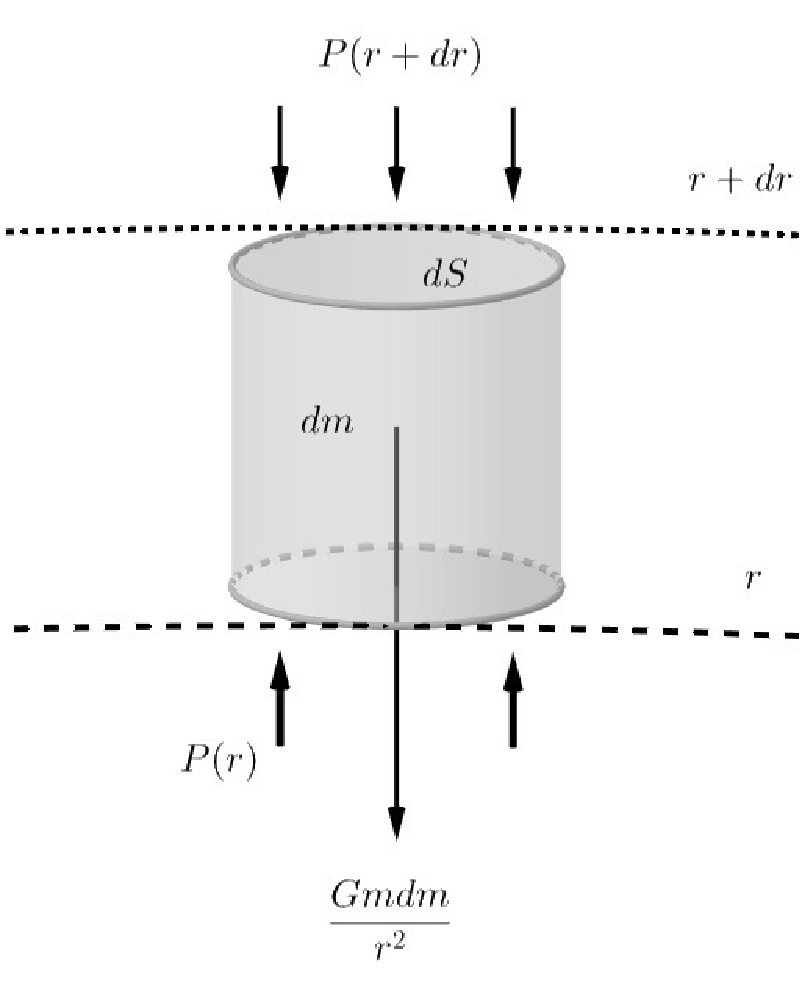
\includegraphics[scale=0.5]{images/cylindre}
	\caption[Cylindre de volume infinitésimal soumis à la force gravitationnelle et à la pression radiative - figure réalisée avec GeoGebra]{Cylindre de volume infinitésimal soumis à la force gravitationnelle et à la pression radiative}
	\label{Fig. A.1}
\end{figure}\bigskip

\begin{figure}[H]
	\centering
	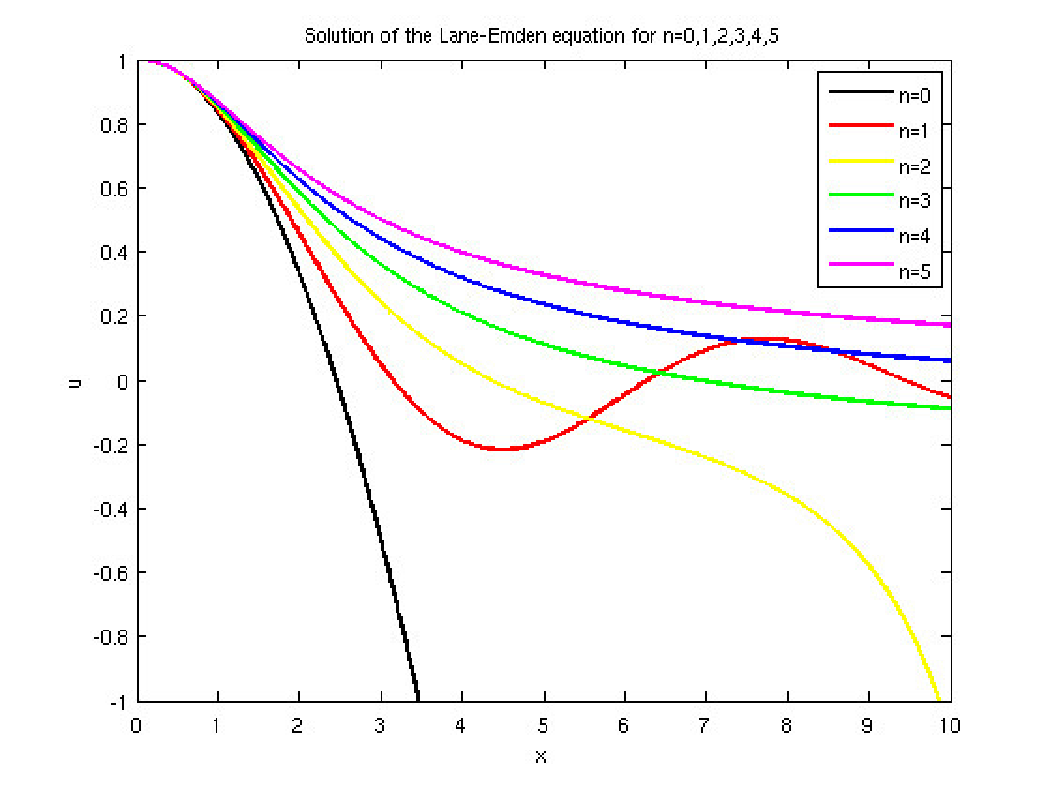
\includegraphics[scale=0.45]{images/graphe_poly}
	\caption[Valeurs de $\theta \left( \xi\right) $ en fonction de l'indice $n$ choisi]{Valeurs de $\theta \left( \xi\right) $ en fonction de l'indice $n$ choisi}
	\addloflink{https://www.mathworks.com/matlabcentral/mlc-downloads/downloads/submissions/23972/versions/22/previews/chebfun/examples/ode/html/LaneEmden.html}
	\label{Fig. A.2}
\end{figure}\bigskip


\chapter{Masse de Chandrasekhar}\label{Annexe B}

Dans les chapitre §\ref{2} et §\ref{3}, nous avons brièvement parlé de la masse de Chandrasekhar. Cette masse limite est la masse maximale que la pression de dégénérescence des électrons peut retenir sans que l'effondrement gravitationnel se poursuive. Elle a été découverte et calculée en 1930 par le physicien indien Chandrasekhar.  Grâce au modèle polytropique que nous avons développé au §\ref{1.2}, nous allons pouvoir obtenir la valeur numérique de cette fameuse limite.\bigskip

Tout d'abord, isolons $\rho_c$ dans l'Eq. \ref{Eq. 1.17}, remplaçons ce résultat dans l'Eq. \ref{Eq. 1.22},  dans cette même équation substituons $\alpha$ par l'Eq. \ref{Eq. 1.20} et réarrangeons les termes, nous obtenons: \begin{equation}\left( \dfrac{GM}{M_{n}}\right)^{n-1} \left( \dfrac{R}{R_{n}}\right)^{3-n}=\dfrac{\left[ \left( n+1\right)K\right]^n}{4\pi G}\label{Eq. 7.1}\end{equation}
avec arbitrairement choisis:
\begin{equation}M_{n}=-\xi_{1}^{2}\left( \dfrac{d\theta}{d\xi}\right)_{\xi_{1}}\label{Eq. 7.2}\end{equation}

\begin{equation}R_{n}=\xi_{1}\label{Eq. 7.3}\end{equation}

De plus, dans l'Eq.\ref{Eq. 7.1}, pour la valeur $n=3$, la masse $M$ est uniquement déterminée par $K$ et indépendante du rayon $R$: 
\begin{equation}M=4\pi M_{3}\left(\dfrac{K}{\pi G}\right)^{3/2}\label{Eq. 7.4}\end{equation}

Ensuite, si $1<n<3$, nous avons de l'Eq.\ref{Eq. 7.1}:
\begin{equation}R^{3-n}\propto\dfrac{1}{M^{n-1}}\label{Eq. 7.5}\end{equation} L'Eq. \ref{Eq. 7.5} nous dit que plus la masse d'un noyau stellaire augmente, plus son rayon diminue.\smallskip 

Nous essayons ici donc de trouver le noyau le plus massif et donc le plus dense qui soit encore en équilibre thermodynamique (§\ref{1.1}); la masse que possède le noyau que nous cherchons est la masse de Chandrasekhar.\smallskip

Le cas limite d'un gaz, composant une étoile, soumis à une énorme pression engendrée par une densité extrême est un gaz relativiste dégénéré. Nous le qualifions de relativiste, car les particules qui le composent sont soumises à de tels niveaux de pression qu'elles atteignent presque la vitesse de la lumière.\smallskip

L'équation d'état polytropique (Eq. \ref{Eq. 1.13}) décrivant ce type de gaz est donné par:\begin{equation}P=K_{2}  \rho^{4/3}\label{Eq.7.6}\end{equation}
avec $K_{2}$ étant déterminé par des lois quantiques et relativistes \autocite{prialnikIntroductionTheoryStellar2009}:
\begin{equation}K_{2}=\dfrac{hc}{8}\left(\dfrac{3}{\pi}\right)^{1/3} \dfrac{1}{m_{H}^{4/3}}\hspace{5pt}\mu_e^{-4/3}\label{Eq. 7.7}\end{equation}
A partir de l'indice adiabatique $\gamma = 4/3$, il est aisé de déterminer l'indice polytropique (Eq. \ref{Eq. 1.14}): $n=3$. De plus, l'Eq. \ref{Eq. 7.4} nous a permis de montrer que pour $n=3$, la masse $M$ est uniquement dépendante de $K$; autrement dit, pour un $K$ donné, il existe une seule masse $M$ possible. Ainsi, si nous substituons $K$ par $K_{2}$ (décrivant le cas limite d'un gaz dégénéré relativiste) dans l'Eq. \ref{Eq. 7.4}, nous obtenons la masse limite de Chandrasekhar: \begin{equation}M_{Ch}=\dfrac{M_{3}\sqrt{1.5}}{4\pi}\left( \dfrac{hc}{Gm_{H}^{4/3}}\right)^{3/2}\hspace{5pt}\mu_{e}^{-2}\label{Eq. 7.8}\end{equation}

En insérant la valeur des constantes l'expression se transforme en:
\begin{equation}M_{Ch}=5.83\hspace{3pt}\mu_{e}^{-2}M_\odot\label{Eq. 7.9}\end{equation}

La variable $\mu_{e}$ décrit la composition chimique d'une étoile. Si le coeur d'une étoile est composé de fer: $\mu_{e}=2.15$; si il est composé de carbone et d'oxygène: $\mu_{e}=2$. La masse de Chandrasekhar n'est donc pas une valeur fixe, elle peut varier un peu en fonction des constituants de l'étoile.\bigskip

Pour $\mu_{e}=2$: 
\begin{equation}M_{Ch}=1.46\hspace{3pt}M_\odot\label{Eq. 7.10}\end{equation}

